\documentclass{article}

\usepackage{graphicx}
\usepackage{rotating}
\usepackage{amsmath}
\usepackage{amssymb}
\usepackage{fancyhdr}
\usepackage{listings}
\usepackage{xcolor}
\usepackage{color}
\usepackage{amsfonts}
\usepackage{textcomp}
\usepackage{float}
\usepackage[sorting=none]{biblatex}
\usepackage[margin=1in]{geometry}
\usepackage[font={small,it}]{caption}
\usepackage{placeins}
\usepackage{xepersian}

%\DeclareMathOperator*{\btie}{\bowtie}
\addbibresource{bibliography.bib}
\settextfont[Scale=1.2]{B-NAZANIN.TTF}
\setlatintextfont[Scale=1]{Times New Roman}
\renewcommand{\baselinestretch}{1.5}
\pagestyle{fancy}
\fancyhf{}
\rhead{تکلیف اول درس مهندسی فناوری اطلاعات}
\lhead{\thepage}
\rfoot{علیرضا ابره فروش}
\lfoot{9816603}
\renewcommand{\headrulewidth}{1pt}
\renewcommand{\footrulewidth}{1pt}
\newcommand{\Lagr}{\mathcal{L}}
\newcommand{\Mod}[1]{\ (\mathrm{mod}\ #1)}
%%%%%%%%%%
\lstset
{
    language=[latex]tex,
    basicstyle=\ttfamily,
    commentstyle=\color{black},
    columns=fullflexible,
    keepspaces=true,
    upquote=true,
    showstringspaces=false,
    morestring=[s]\\\%,
    stringstyle=\color{black},
}
%%%%%%%%%%
%beginMatlab
\definecolor{mygreen}{RGB}{28,172,0} % color values Red, Green, Blue
\definecolor{mylilas}{RGB}{170,55,241}
%endMatlab
\begin{document}
%beginMatlab
\lstset{language=Matlab,%
    %basicstyle=\color{red},
    breaklines=true,%
    morekeywords={matlab2tikz},
    keywordstyle=\color{blue},%
    morekeywords=[2]{1}, keywordstyle=[2]{\color{black}},
    identifierstyle=\color{black},%
    stringstyle=\color{mylilas},
    commentstyle=\color{mygreen},%
    showstringspaces=false,%without this there will be a symbol in the places where there is a space
    numbers=left,%
    numberstyle={\tiny \color{black}},% size of the numbers
    numbersep=9pt, % this defines how far the numbers are from the text
    emph=[1]{for,end,break},emphstyle=[1]\color{red}, %some words to emphasise
    %emph=[2]{word1,word2}, emphstyle=[2]{style},    
}
%endMatlab
\begin{titlepage}
\begin{center}

\includegraphics[width=0.4\textwidth]{figures/IUT Logo.png}\\
        
\LARGE
\textbf{دانشگاه صنعتی اصفهان}\\
\textbf{دانشکده مهندسی برق و کامپیوتر}\\
        
\vfill
        
\huge
\textbf{عنوان: تکلیف چهارم درس ریزپردازنده}\\
        
\vfill
        
\LARGE
\textbf{نام و نام خانوادگی: علیرضا ابره فروش}\\
\textbf{شماره دانشجویی: 9816603}\\
\textbf{نیم\,سال تحصیلی: پاییز 1400}\\
\textbf{مدرّس: دکتر عارف کریمی افشار}\\
\end{center}
\end{titlepage}


%\tableofcontents
\newpage


%1
\section{}
$
m = (00110010)_2 = (50)_{10} \\
p = 23, q = 19 \\
n = pq = 23 \times 19 = 437 \\
z = (p-1)(q-1) = 22 \times 18 = 396 \\
e = 97 \Rightarrow  e < n,\: (e, z) = 1 \\
d = 49 \Rightarrow ed \equiv 1 (mod\:z) \\ \\
c = (m ^ e \equiv 1 (mod \: n)) \Rightarrow c = 335 \\
m = (c ^ d \equiv 1 (mod \: n)) \Rightarrow m = 50 \\ \\
K^+ = e = 97 \\
K^- = d = 49 \\
$


%2
\section{}
\lr{Trudy} می‌تواند به سیستم نفوذ کند و محتوای ارسال شده را تغییر دهد. به این صورت که $M$ و $H(M) + S$ را از هم جدا می‌کند. سپس با محاسبه‌ی \lr{hash}ِ پیامِ $M$ و حذف آن از $H(M)+S$ (به شکل $H(M) + S - H(M)$) به \lr{shared secret} دست پیدا می‌کند. سپس پیام مورد نظر خود ($M^{\prime}$) را به همراه $H(M^{\prime})$ و $S$ برای فرد به شکل
$\left( M^{\prime}, H(M^{\prime}) + S \right)$
ارسال می‌کند. با اینکه این پروتکل قابلیت نفوذ دارد اما به هر حال نمودار استخراج و \lr{Authentication}ِ پیام به صورت زیر است.
\begin{figure}[H]
    \centering
    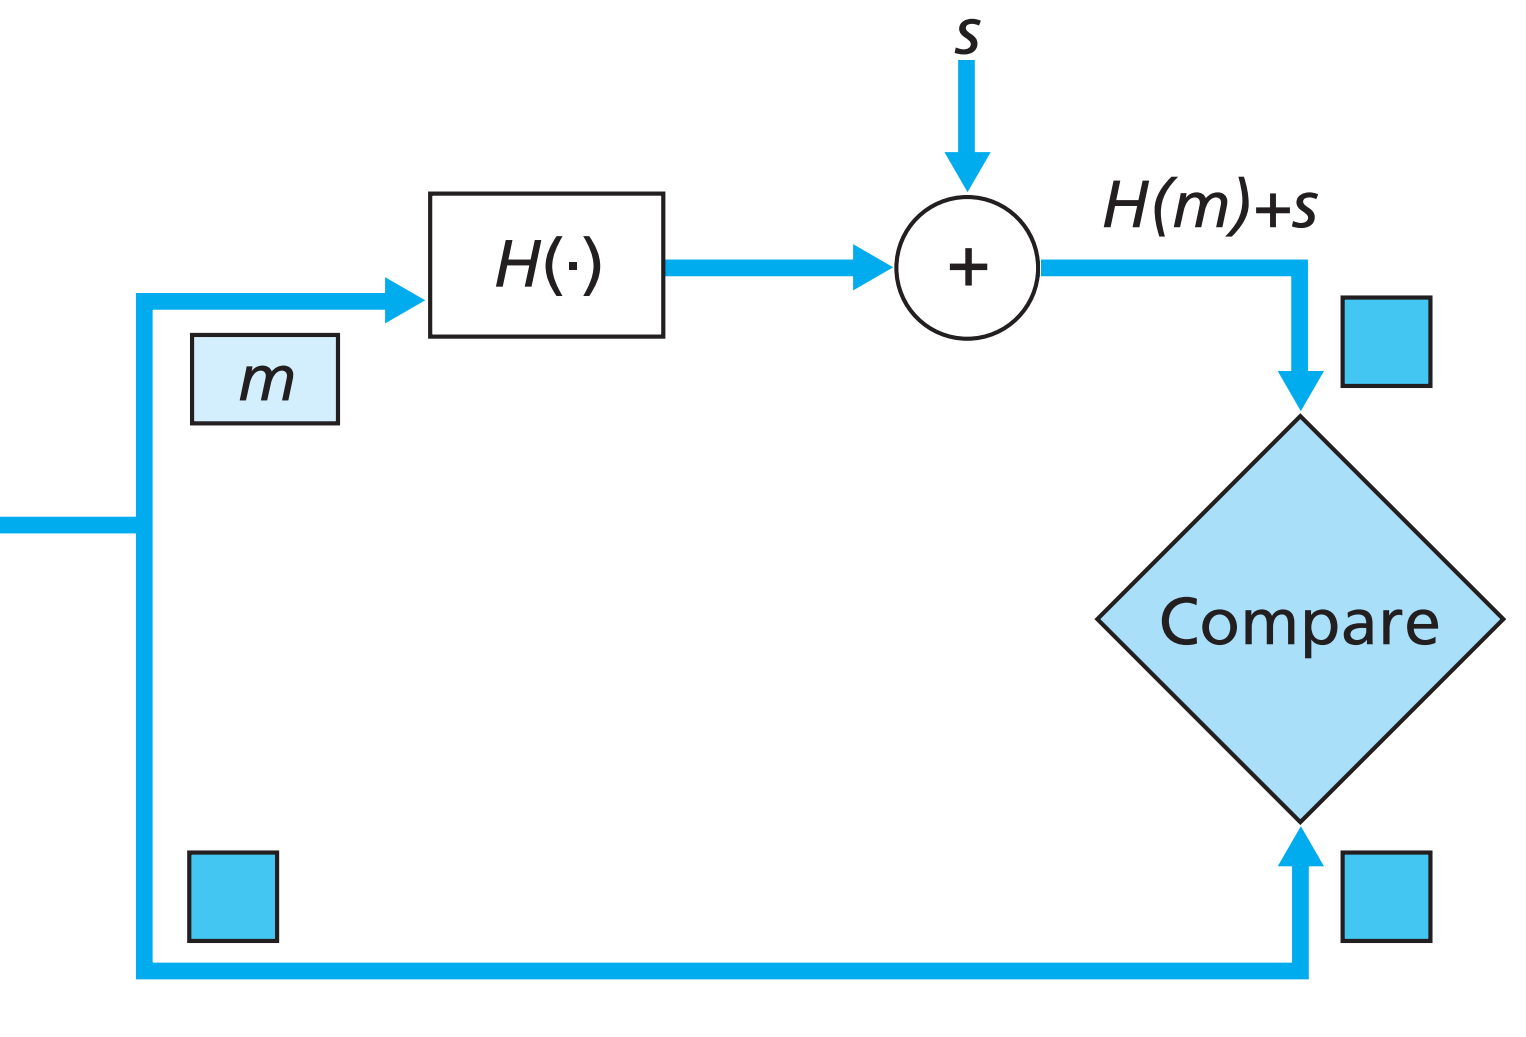
\includegraphics[width=0.50\textwidth]{figures/1.png}
    \caption
	{
نمودار رمزگشایی پیام
	}
    \label{fig:fig1}
\end{figure}


%3
\section{}
اول از هرچیز امضای \lr{message digest} با کلید خصوصی (\lr{private key}) صورت می‌گیرد، نه کلید عمومی (\lr{public key}). به دلیل پیچیدگی محاسباتی عملیات رمزنگاری و رمزگشایی، کل پیام را رمز نمی‌کنیم و فقط \lr{digest}ش را رمز می‌کنیم.

%4
\section{}
هزاران نفر قصد دارند پیام \lr{Alice} را دریافت کنند و \lr{Alice} آماده است که پیام را به هر متقاضی بفرستد. برای تضمین صحت پیام، \lr{Alice} می‌تواند ابتدا \lr{hash}ِ پیام را با \lr{private key}ِ خود رمز کند و همراه پیام
($(m, K_{A}^{-}(H(m)))$)
به هر یک از متقاضیان بفرستد. چون \lr{Alice} تنها کسی است که \lr{private key} خود را دارد و پیامی که با \lr{private key} رمز شده است تنها با \lr{public key} نظیر همان \lr{private key} قابل رمزگشایی است، در این صورت هر یک از دریافت‌کننده‌های پیام می‌توانند صحت این پیام را احراز کنند. به این صورت که هر یک از دریافت‌کننده‌ها $K_{A}^{-}(H(m))$ و $m$ را از هم جدا می‌کند. سپس با استفاده از \lr{public key}ِ \lr{Alice} $H(m)$ را به شکلِ
$H(m) = K_{A}^{+}(K_{A}^{-}(H(m)))$
به دست می‌آورد. در نهایت با گرفتن \lr{hash} از $m$ِ جدا شده و بررسی برابریِ آن با $H(m)$ به دست آمده در مرحله‌ی قبل صحت پیام احراز می‌شود. توجه شود که برای دستیابی به صحت می‌توانستیم به جای مکانیزم امضای دیجیتال از \lr{MAC} استفاده کنیم. اما در این حالت \lr{Alice} باید به ازای هر دریافت‌کننده
$(m, H(m + s))$
را محاسبه کند که خود این کار با توجه به تعداد زیاد دریافت‌کننده‌های پیام می‌تواند \lr{overhead} قابل توجهی داشته باشد و همچنین لازم بود که به ازای هر دریافت‌کننده یک \lr{shared secret} داشته باشد که مدیریت آن‌ها می‌تواند ساده نباشد. \\
پس در این جا استفاده از \lr{digital-signature-based integrity scheme} نسبت به \lr{MAC algorithm scheme} بهتر است.


%5
\section{}
در اینجا \lr{Trudy} نقش \lr{Man-in-the-middle} را دارد و $N_a$ و $E_k(N_b)$ و $E_k(N_a)$ و $N_b$ را از طرف خود برای \lr{Bob} و \lr{Alice} می‌فرستد و به این صورت \lr{Authenticate} می‌شود.




%6
\section{}
الگوریتم \lr{SSL handshake} به صورت زیر است.

\begin{enumerate}
	\item \lr{Bob} لیستی از الگوریتم‌هایی که از آن‌ها پشتیبانی می‌کند را به همراه \lr{nonce} به \lr{Alice} می‌فرستد.
	\item \lr{Alice} بین لیست الگوریتم‌های پیشنهادی یکی را انتخاب می‌کند و آن را به همراه \lr{certificate} و \lr{nonce} می‌فرستد.
	\item \lr{Bob} \lr{certificate} را اعتبارسنجی می‌کند، \lr{public key}ِ \lr{Alice} را استخراج می‌کند، \lr{pre\_master\_secret} را تولید می‌کند، با \lr{public key}ِ \lr{Alice} آن را رمز می‌کند و برای \lr{Alice} می‌فرستد.
	\item \lr{Bob} و \lr{Alice} به طور مستقل رمز و کلیدهای \lr{MAC} را از \lr{pre\_master\_secret} و \lr{nonce}ها محاسبه می‌کنند.
	\item \lr{Bob} یک \lr{MAC} از همه‌ی پیام‌های \lr{handshake} می‌فرستد.
	\item \lr{Alice} یک \lr{MAC} از همه‌ی پیام‌های \lr{handshake} می‌فرستد.
\end{enumerate}

اگر \lr{Trudy} خود را \lr{Alice} جا زده باشد، در گام 6 باید یک \lr{MAC} ($H(m+s)$) از همه‌ی پیام‌های \lr{handshake} به \lr{Bob} بفرستد و از آن‌جایی که \lr{shared secret} را ندارد نمی‌تواند \lr{MAC} را به درستی محاسبه کند. پس \lr{Bob} در ای ن گام متوجه می‌شود که با \lr{Alice} در ارتباط نیست.

%7
\section{}
فایروال‌های \lr{stateless} پکت‌ها را به طور مستقل از یک دیگر در نظر می‌گیرند. در حالی که فایروال‌های \lr{stateful} اطلاعات مربوط به پکت‌های قبلا منتقل شده را ذخیره می‌کنند. برای مثال حالتی که \lr{Attacker} بدون آغاز کردن یک \lr{connection} (که با \lr{Syn} است) \lr{Ack} می‌فرستد. اگر در این سمت یک فایروال \lr{stateful} وجود داشته باشد این تغییر رفتاری را متوجه می‌شود. به طور کلی تفاوت فایروال \lr{stateless} و \lr{stateful} از قرار زیر است:
\begin{figure}[H]
    \centering
    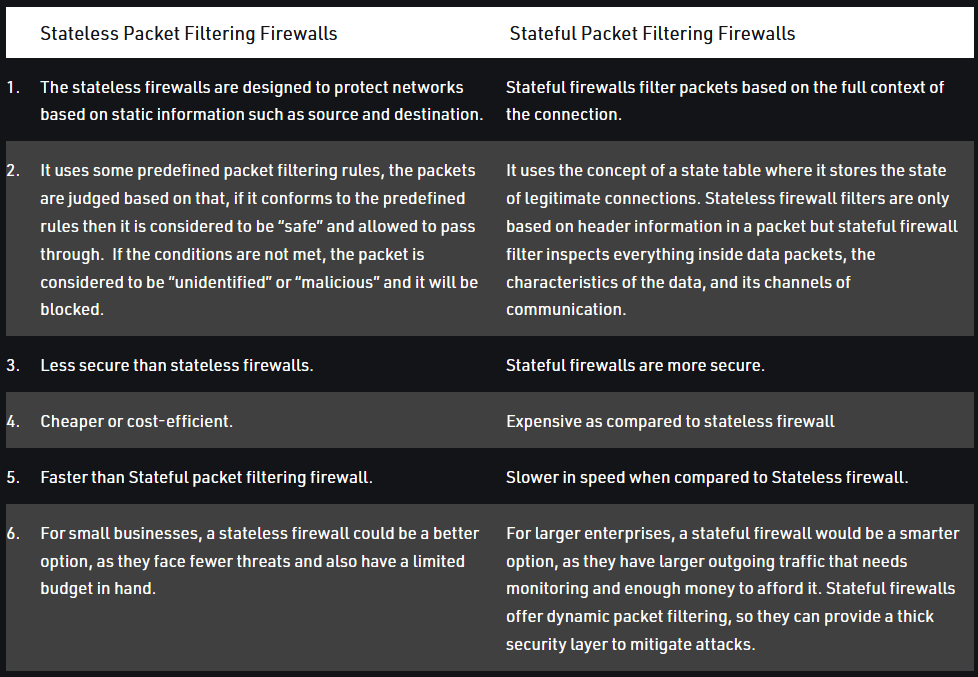
\includegraphics[width=1\textwidth]{figures/2.png}
    \caption
	{}
    \label{fig:fig1}
\end{figure}





%8
\section{}
\lr{Attacker} با \lr{IV}ِ شناخته شده به عنوان پایه شروع می‌کند و مکررا \lr{sub-attack} را اعمال می‌کند تا همه‌ی کلیدواژه‌های در \lr{secret key}ِ را بازیابی کند. \lr{cryptoanalyst} به اولین کلمه‌ی خروجی از تعداد زیادی \lr{RC4 stream} به همراه \lr{IV}ای که برای تولید هر کدام از آن‌ها استفاده شده است نیاز دارد؛ و اولین کلمه‌ی پیام در اکثر پکت‌ها یک ثابت شناخته شده است. این الزامات به طور خودکار برآورده می‌شوند.

با حدود 60 \lr{IV}ی این‌چنینی، \lr{Attacker} می‌تواند کلید را با احتمال موفقیت قابل قبول به دست آورد. تعداد پکت‌های مورد نیاز برای دستیابی به آن تعداد \lr{IV} دقیقا به \lr{IV}هایی که فرستنده استفاده می‌کند بستگی دارد. همچنین استاندارد \lr{802.11b} طریقه‌ی پیاده‌سازی این \lr{IV}ها را مشخص نکرده است. روش معمول استفاده از یک شمارش‌گر برای تولید آن‌هاست. اگر شمارش‌گر از 0 شروع نشود، \lr{Attacker} استراتژی مشابه دارد. اگر \lr{Attacker} دو بایت اول \lr{secret key} را در نظر بگیرد، برای هر بایت \lr{IV}ِ ابتدایی، تقریبا  
4 چینش از دو بایتی که جایگشت مورد نیاز برای بازیابی یک بایت شامل کلید را می‌سازد وجود دارد.

\lr{Fluhrer S.}، \lr{Mantin I.} و \lr{Shamir A.} در \lr{Attacks on RC4 and WEP} توضیح می‌دهند که $x$ کلمه‌ی اول \lr{KSA key} شناخته شده است. این قضیه باعث می‌شود که بتوان $x$ دور اول \lr{KSA} را شبیه‌سازی کنیم و جایگشت $S_{x-1}$ و اندیس $i_{x-1}$ در آن نقطه را محاسبه کنیم. مقدار بعدی $i$ نیز شناخته شده است ($i_x = x$)، اما مقدار بعدی $j(j_x)$ به کلیدواژه‌ی هدف $K\left[ x \right]$ وابسته است (چون
$j_x = j_x - 1 + S_x - 1 \left[ x \right] + K\left[ x \right]$
) و در نتیجه هر یک از مقادیر $j_x$ و $K\left[x\right]$ به سادگی از دیگری قابل بازیابی هستند. در نتیجه به ازای $S_x\left[x\right]$ داده شده می‌توان حساب کرد که کدام مقدار در جایگاه $j_x$ در جایگشت شناخته شده‌ی $S_{x-1}$ قرار داشته است و از طریق برعکس کردن این جایگشت می‌توان $j_x$ را بازیابی کرد. برای توضیح بیشتر به منبع مراجعه کنید.






%%%%%%%%%%%%%%%%%%%%%%%%%%%%%%%%%%%
%%%%%%%%%%%%%%%%%%%%%%%%%%%%%%%%%%%
%%%%%%%%%%%%%%%%%%%%%%%%%%%%%%%%%%%






\section*{منابع}
\renewcommand{\section}[2]{}%
\begin{thebibliography}{99} % assumes less than 100 references
%چنانچه مرجع فارسی نیز داشته باشید باید دستور فوق را فعال کنید و مراجع فارسی خود را بعد از این دستور وارد کنید


\begin{LTRitems}

\resetlatinfont

\bibitem{b1} Stošić, Lazar, and Milena Bogdanović. "RC4 stream cipher and possible attacks on WEP." Editorial Preface 3.3 (2012).
\end{LTRitems}

\end{thebibliography}


\end{document}
